\begin{figure*}[t]
  \centering
  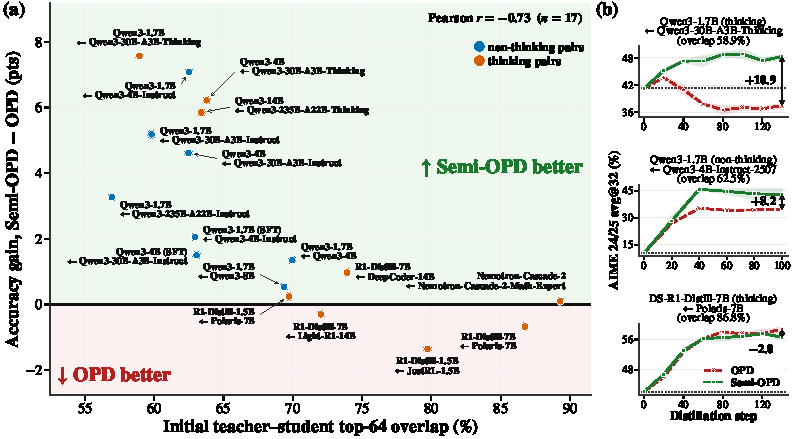
\includegraphics[width=0.95\linewidth]{figures/fig_overlap_combo.pdf}
  \vspace{-0.5em}
  \caption{
\textbf{当初始教师-学生重叠度较低时，Semi-OPD优于标准OPD。}
\textbf{(a)} 17对模型在从1.5B到235B规模范围内，涵盖思维模式与非思维模式以及多个模型家族的初始前64重叠度下的准确率提升情况，皮尔逊相关系数为$r=-0.73$。准确率提升是指Semi-OPD与OPD准确率曲线之间的面积差除以两者共享的训练周期，对AIME~24/25/26和HMMT~Feb~26取平均。
\textbf{(b)}~三个重叠度逐步增加的模型对的训练曲线（AIME~24/25平均@32，3个种子的均值）。在低重叠度下，Semi-OPD表现优于OPD，而OPD甚至可能出现性能下降；在高重叠度下，Semi-OPD可能略微落后。}
  \label{fig:overlap}
  \vspace{-1em}
\end{figure*}



\section{引言}
\label{sec:intro}

同策略蒸馏（OPD）已成为一种有效的方法，用于将教师语言模型（LM）的能力迁移至学生语言模型~\citep{agarwal2024policy, gu2024minillm, lu2025onpolicydistillation, xiao2026mimov2flashtechnicalreport, xu2026deepseek}。它通过在通过同策略采样获得的学生轨迹上提供来自教师语言模型的稠密 token 级信号，缓解了传统知识蒸馏中的训练-推理分布不匹配问题，即曝光偏差。 

尽管前景乐观，近期的研究揭示了同策略蒸馏（OPD）的若干缺陷：\citep{luo2026demystifying, yang2026eos, fu2026revisiting, yu2026mismatch} 发现同策略的滚动采样往往导致生成序列过长，并陷入自我修正环路，耗尽生成预算却无法输出结束符（EOS token）；\citep{zhang2026fast,ziheng2026less, liu2026prefix} 发现对学生滚动采样中后期 token 的监督通常无益，截断至短前缀即可满足需求；而 \citep{xu2026pass,jiang2026trajectory} 也发现，一旦学生模型确定了错误的推理方向，后续偏离方向的延续会产生不可靠的监督信号并浪费计算资源。这些缺陷引出了我们核心的问题：

\begin{center}
\vspace{-0.5em}
\emph{同策略采样对于任意教师-学生配对的蒸馏是否总是有益的？}
\vspace{-0.5em}
\end{center}



为回答这一问题，我们提出了一种简单且高效的替代方法——半同策略蒸馏（Semi-OPD），其中在任何训练开始前，仅从初始学生模型中采样一次轨迹，并在整个蒸馏过程中重复使用，从而使得轨迹生成和教师Logit生成均为离线进行。尽管轨迹来源固定，但目标与同策略蒸馏（OPD）相同，且学生模型的对数概率，因此每个token的优势值，会在每一步使用当前参数重新计算。

我们在17组教师-学生配对上进行了评估，涵盖15亿至2350亿参数的三种模型家族，在思考模式与非思考模式下均进行了测试，覆盖了OPD文献中最常用的师生配对。我们发现，Semi-OPD在其中14组上优于OPD，准确率最高提升达+13.6\%，训练速度最快提升11.4$\times$，如图~\ref{fig:speedup}所示；而在其余三组上，性能相当（差距在0.1\%--2.6\%之间）。  
这一现象促使我们进一步探究如何在Semi-OPD与OPD之间进行选择，以及为何Semi-OPD通常表现更优。


\noindent \textbf{如何在半监督同策略蒸馏（Semi-OPD）与同策略蒸馏（OPD）之间进行选择。}
我们发现，Semi-OPD相较于OPD的收益与初始教师模型和学生模型之间的对齐程度密切相关，这一对齐程度可通过输出token上的教师-学生前$k$名重叠比率来量化，如图~\ref{fig:overlap}a所示。
图~\ref{fig:overlap}b中的准确率演化曲线进一步表明：(1) 当该重叠比率较低时，持续从不断演化的学生模型中重新生成轨迹会使得训练逐渐偏离教师模型的轨迹，此时严格的同策略性反而适得其反；(2) 仅当教师模型与学生模型具有较高的重叠比率时，OPD才具有优势。 


\noindent \textbf{为什么同策略蒸馏（OPD）通常表现不如半同策略蒸馏（Semi-OPD）。} 我们的实证研究表明，有效的蒸馏需要在学生和教师两个方面都具备“同策略性”，前者可缓解曝光偏差，后者决定了蒸馏信号的有效性。OPD 改进了前者，但可能削弱了后者。

具体而言，对于对齐不充分的样本对，随着上下文长度的增长，OPD 生成的学生轨迹相对于教师会变得越来越异策略。这种问题无法通过简单的截断来解决，因为我们实证表明，覆盖不同推理阶段的监督信号至关重要。

相比之下，Semi-OPD 在初始学生轨迹上通常在较短的上下文中进行蒸馏，同时覆盖完整的轨迹，因此更加稳定。换句话说，Semi-OPD 以牺牲部分学生同策略性为代价，换取了更强的教师同策略性，这一点也与我们的观察一致：Semi-OPD 使学生接触到更多教师所偏好的 token。


我们旨在激发社区重新思考使用OPD的时机，并在有意义的情景下研究更强大的OPD变体。我们的工作主要收获总结如下：


\begin{itemize}[leftmargin=1.2em]
\vspace{-1em}
\item OPD仅在教师-学生对的输出token具有高重叠度时才有效；对于非对齐对，Semi-OPD在准确率和训练效率方面都是更好的选择。

\item 有效的蒸馏需要同时满足学生模型在训练轨迹上的同策略性以及与教师模型的接近性；而OPD更侧重前者，可能牺牲后者。

\item 鉴于目标领域和初始师生对，应根据测得的重叠比例来决定选择OPD还是半监督OPD，而不是盲目选择OPD。

\item 未来对OPD的研究应仔细选择师生配对，以确保实验情景具有意义。

\end{itemize}

